\documentclass[oneside,14pt]{extarticle}
\usepackage{cmap}
\usepackage[utf8]{inputenc}
\usepackage[english,ukrainian]{babel}
\usepackage{graphicx}
\usepackage{geometry}
\usepackage{listings}
\usepackage{float}
\usepackage{amsmath}
\usepackage{subfig}
\usepackage{tempora}
\geometry{
	a4paper,
	left=20mm,
	right=20mm,
	top=15mm,
	bottom=15mm,
}
\lstset{
	language=c,
	tabsize=4,
	keepspaces,
	showstringspaces=false,
	frame=single,
	breaklines,
	language=C,
}
\graphicspath{ {./pictures} }
\setlength{\parindent}{4em}

\newcommand\subject{Безпека програм та даних}
\newcommand\lecturer{к.т.н., доцент кафедри ПЗ\\Сенів М.М.}
\newcommand\teacher{к.т.н., доцент кафедри ПЗ\\Сенів М.М.}
\newcommand\mygroup{ПЗ-42}
\newcommand\lab{2}
\newcommand\theme{Створення програмного засобу для забезпечення цілісності інформації}
\newcommand\purpose{Ознайомитись з методами криптографічного забезпечення
	цілісності інформації, навчитись створювати програмні засоби для
	забезпечення цілісності інформації з використанням алгоритмів хешування}

\begin{document}
\begin{normalsize}
	\begin{titlepage}
		\thispagestyle{empty}
		\begin{center}
			\textbf{МІНІСТЕРСТВО ОСВІТИ І НАУКИ УКРАЇНИ\\
				НАЦІОНАЛЬНИЙ УНІВЕРСИТЕТ "ЛЬВІВСЬКА ПОЛІТЕХНІКА"}
		\end{center}
		\begin{flushright}
			\textbf{ІКНІ}\\
			Кафедра \textbf{ПЗ}
		\end{flushright}
		\vspace{80pt}
		\begin{center}
			\textbf{ЗВІТ}\\
			\vspace{10pt}
			до лабораторної роботи № \lab\\
			\textbf{на тему}: <<\textit{\theme}>>\\
			\textbf{з дисципліни}: <<\subject>>
		\end{center}
		\vspace{80pt}
		\begin{flushright}
			
			\textbf{Лектор}:\\
			\lecturer\\
			\vspace{28pt}
			\textbf{Виконав}:\\
			
			студент групи \mygroup\\
			Коваленко Д.М.\\
			\vspace{28pt}
			\textbf{Прийняв}:\\
			
			\teacher\\
			
			\vspace{28pt}
			«\rule{1cm}{0.15mm}» \rule{1.5cm}{0.15mm} 2024 р.\\
			$\sum$ = \rule{1cm}{0.15mm}……………\\
			
		\end{flushright}
		\vspace{\fill}
		\begin{center}
			\textbf{Львів — 2024}
		\end{center}
	\end{titlepage}
		
	\begin{description}
		\item[Тема.] \theme.
		\item[Мета.] \purpose.
	\end{description}

    \section*{Лабораторне завдання}
    Створити програмну реалізацію алгоритму хешування MD5. Програмна реалізація повинна виводити значення хешу як для рядка,
    заданого в полі вводу, так і для файлу. Результат роботи програми повинен
    відображатись на екрані з можливістю наступного запису в файл. Крім того
    програма повинна мати можливість перевірити цілісність будь-якого файлу за
    наявним файлом з MD5 хешем, записаним у шістнадцятковому форматі. У звіті
    навести протокол тестування і роботи програми та зробити висновки.
    
	\section*{Хід роботи}
	
	\subsection*{Виконання програми}
	\begin{figure}[H]
		\centering
		\begin{minipage}{0.45\textwidth}
			\centering
			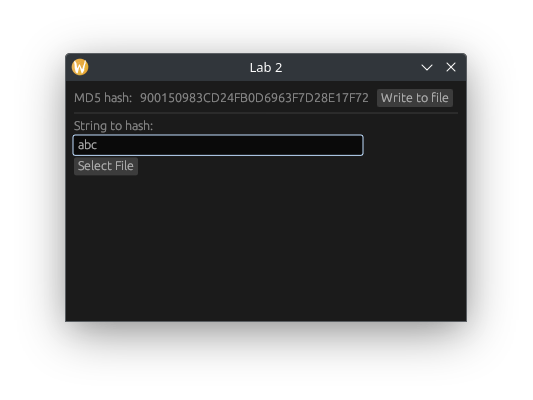
\includegraphics[scale=0.6]{1}
			\caption{Хешування стрічки}
		\end{minipage}
		\hfill
		\begin{minipage}{0.45\textwidth}
			\centering
			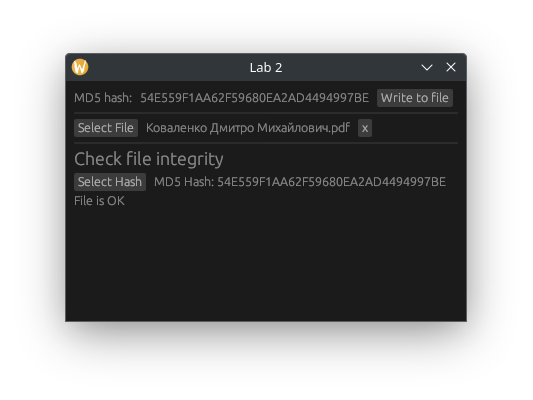
\includegraphics[scale=0.6]{2}
			\caption{Перевірка цілісності файлу}
		\end{minipage}
	\end{figure}
	
	\subsection*{Код програми}
	Файл \textit{main.rs}:
	{\small	\lstinputlisting{src/main.rs}}
	
	\section*{Висновки}
	Під час виконання лабораторної роботи я ознайомився з методами криптографічного забезпечення цілісності інформації, навчився створювати програмні засоби для
	забезпечення цілісності інформації з використанням алгоритмів хешування.
	    
\end{normalsize}
\end{document}
